\begin{figure}[!htb]
    \begin{center}
    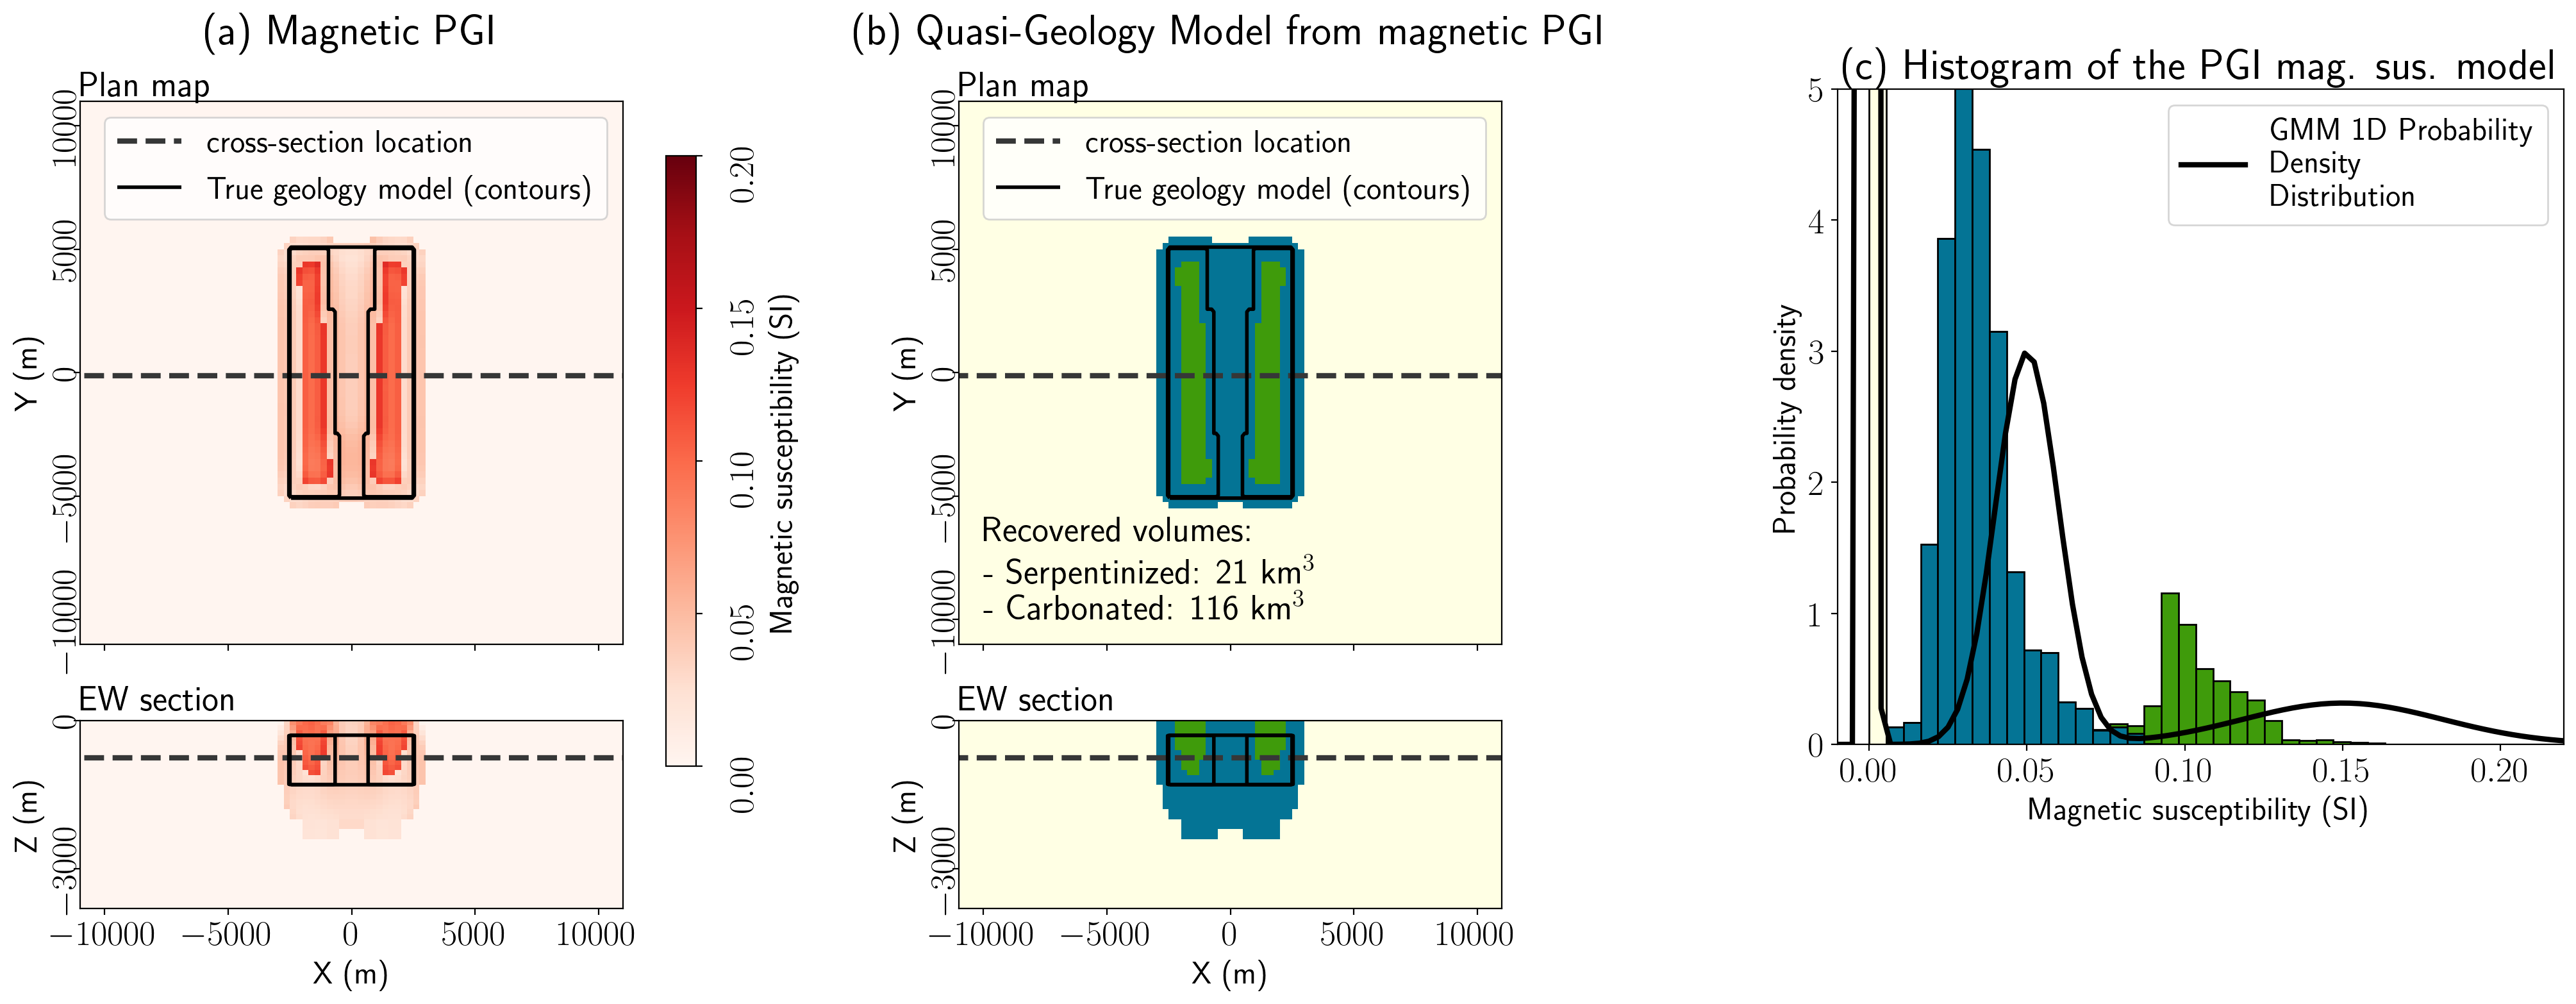
\includegraphics[width=0.9\textwidth]{figures/Single-Physics-PGI-Magnetic.png}
    \end{center}
\caption{
    Results from inverting the magnetics data with the PGI framework. (a) Magnetic susceptibility model, (b) associated quasi-geology model, and (c) histogram of the recovered magnetic susceptibility values.
}
\label{fig:single-physics-pgi-magnetics}
\end{figure}
